%Simple slideshow for the BIRC lobby
%each slide will be shown for a fixed period of time
%Duplicate slides to increase duration
%R. Hancock 9/26/17

\documentclass[aspectratio=169]{beamer}
\usepackage{lmodern}

\usetheme{Rochester}
%gets rid of bottom navigation bars
\setbeamertemplate{footline}[frame number]{}

%gets rid of bottom navigation symbols
\setbeamertemplate{navigation symbols}{}
\setbeamercolor{structure}{fg=beamer@uconnnavy}
\definecolor{beamer@uconnnavy}{rgb}{0.0,0.0549,0.1843}

\makeatletter
    \newenvironment{withoutheadline}{
        \setbeamertemplate{headline}[default]
        \def\beamer@entrycode{\vspace*{-\headheight}}
    }{}
\makeatother

%gets rid of footer
%will override 'frame number' instruction above
%comment out to revert to previous/default definitions
\setbeamertemplate{footline}{}
\begin{document}


%%% Logo
\begin{withoutheadline}\begin{frame}

	\begin{center}
		
\includegraphics[width=\textwidth]{img/logo.png}
	\end{center}
\end{frame}\end{withoutheadline}


%%% Lepley
\begin{frame}
	\frametitle{Adam Lepley}
	\framesubtitle{Clinical Education Coordinator, Athletic Training Program\\ \textit{Department of Kinesiology}}

	\begin{columns}[T]
		\begin{column}{.25\textwidth}
			% \begin{block}{}
			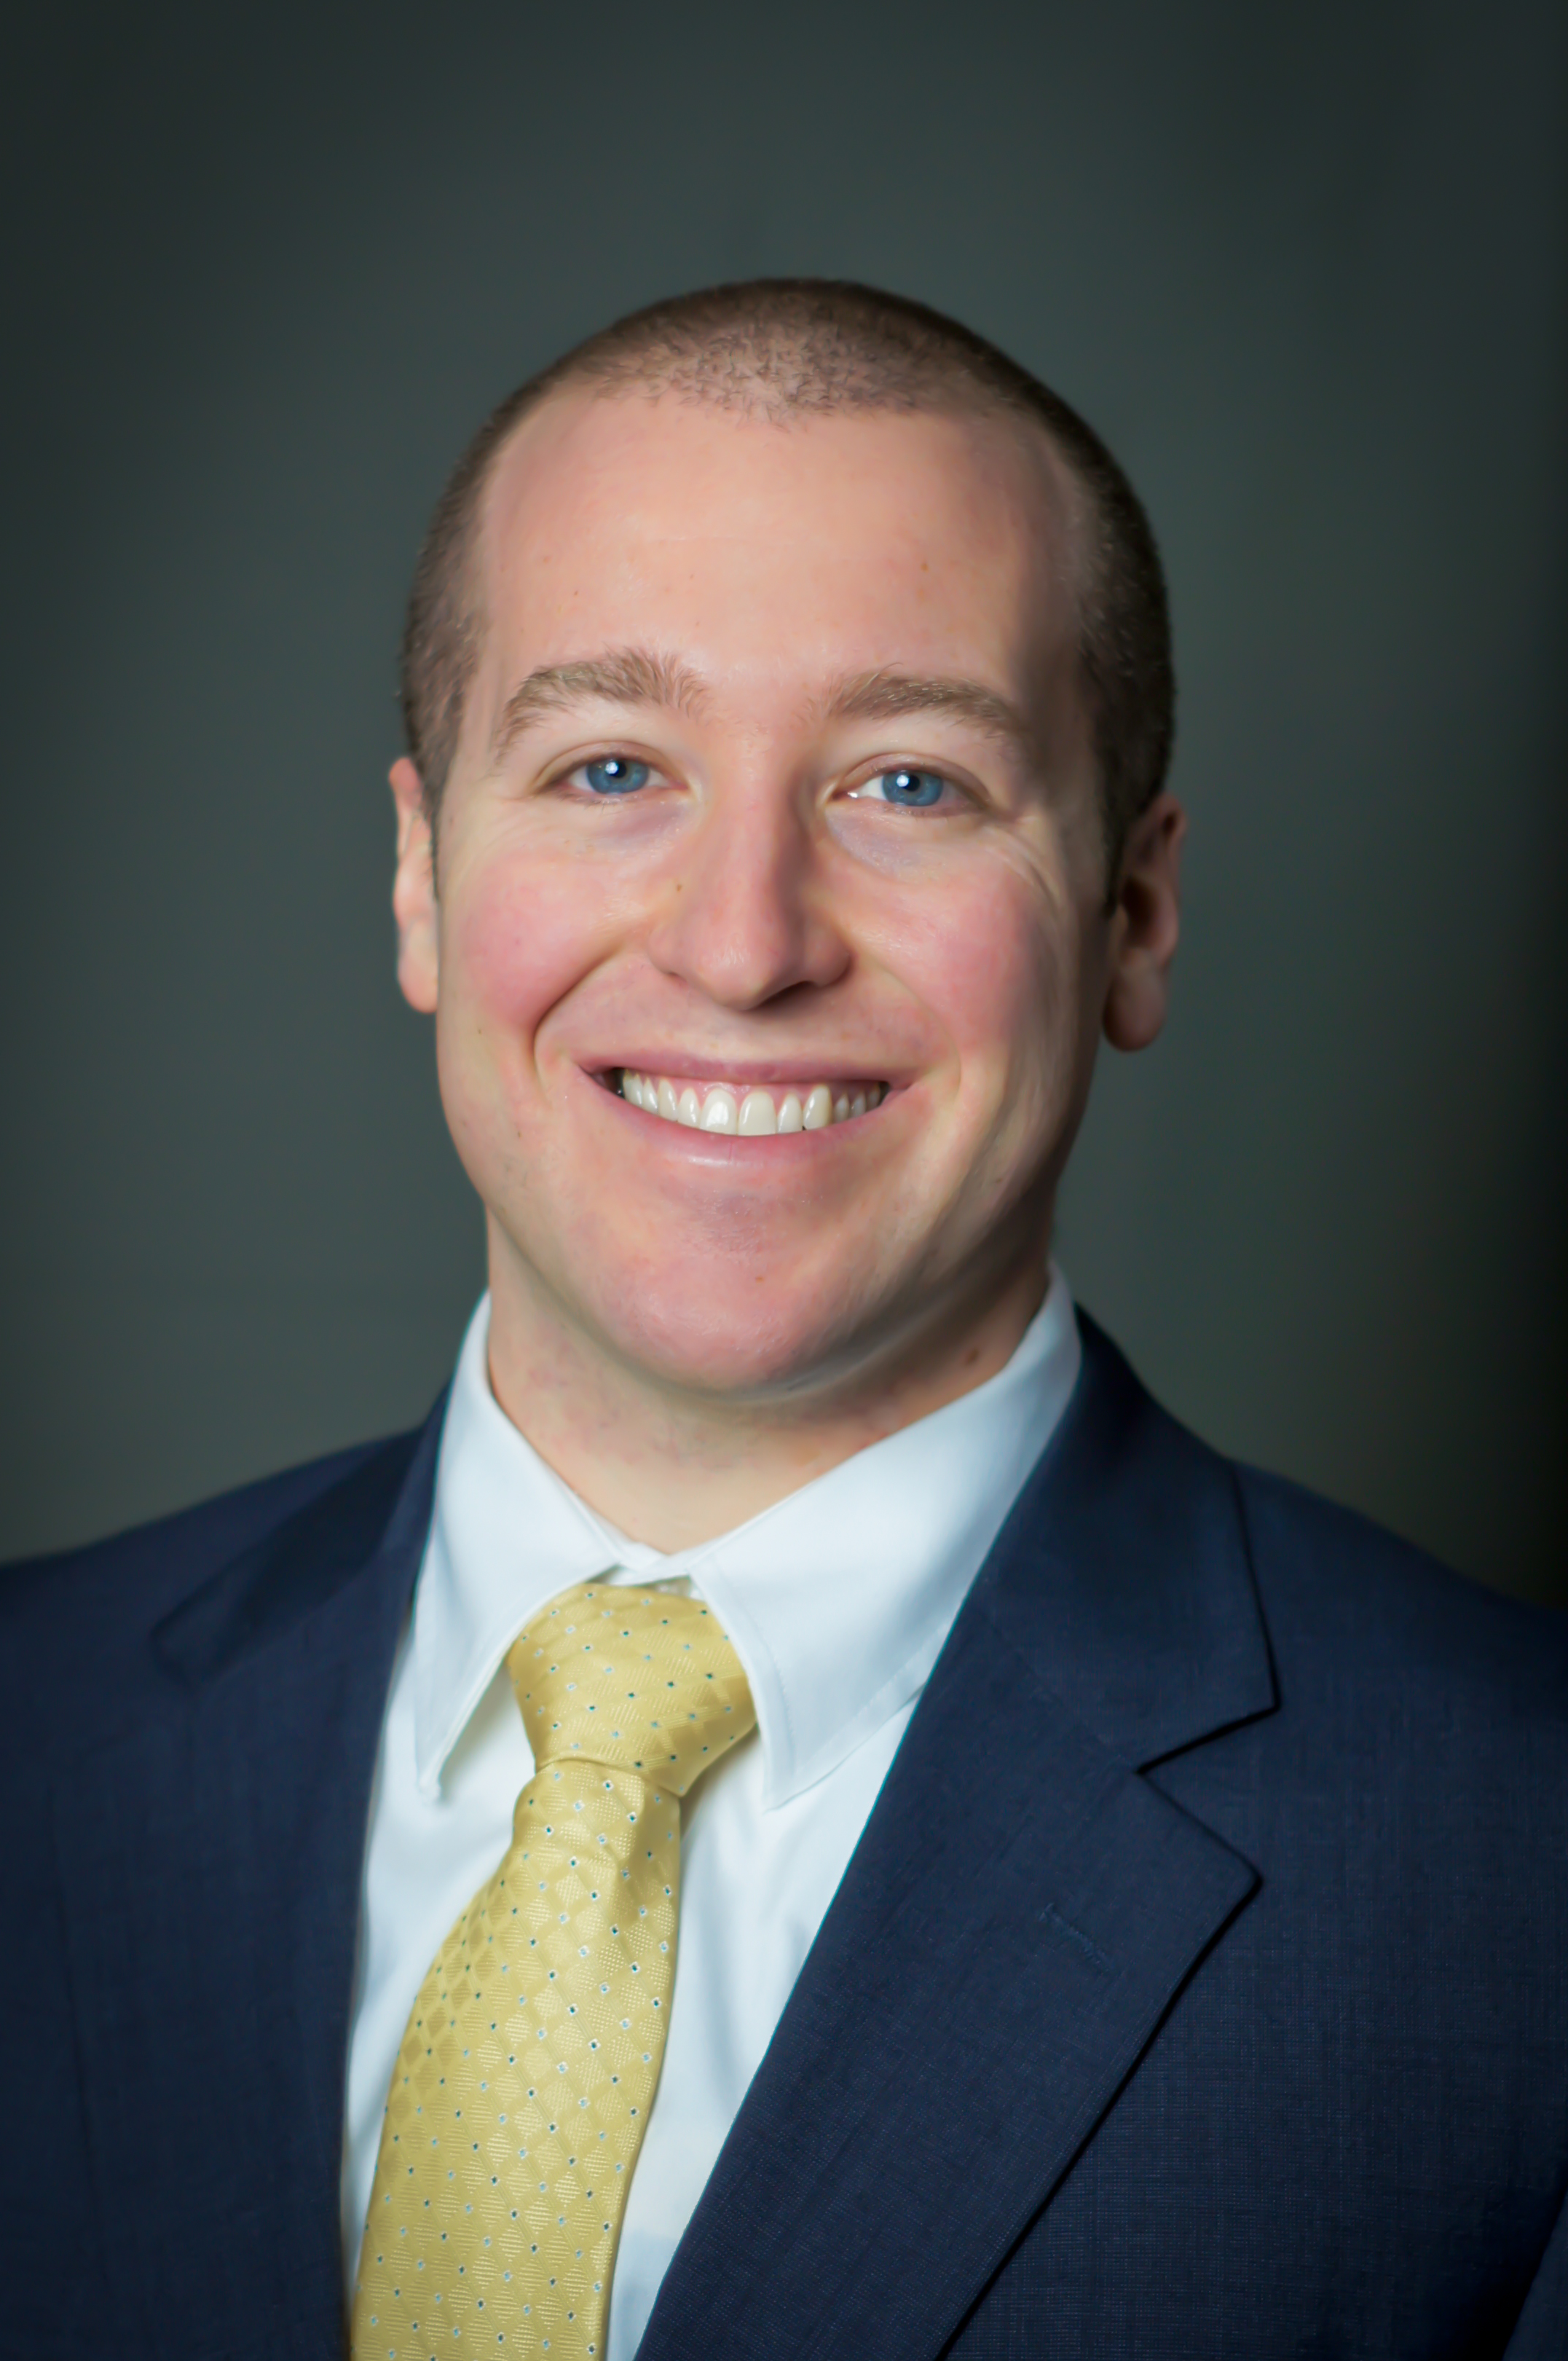
\includegraphics[width=\textwidth]{img/lepley.jpg}
			%  \end{block}
		\end{column}

		\begin{column}{.75\textwidth}
			Dr. Adam Lepley's research interests are focused on maximizing clinical outcomes following musculoskeletal injury, specifically involving the knee. In particular, Dr. Lepley examines the neural contributions to muscle dysfunction and their involvement in lower extremity biomechanical and self-reported disability. The overall goal of this research is to identify the origins of persistent neuromuscular dysfunction for the purpose of developing targeting rehabilitation strategies that are capable of maintaining long-term joint health following acute injury.
		\end{column}
	\end{columns}
\end{frame}

%%% Lepley 2

\begin{frame}
	\frametitle{Contributions of Cortical Activation and Neural Excitability on Quadriceps Muscle Function in Patients with ACL Reconstruction}

	The overall objective of this investigation is to examine differences in neural (brain sctivation/fMRI, motor cortex excitability (TMS), spinal-reflex excitability) and morphological characteristics (cross sectional area) of quadriceps muscle function between participants with anterior cruciate ligament reconstruction (ACLR) and healthy matched controls. 
	
	\begin{center}
		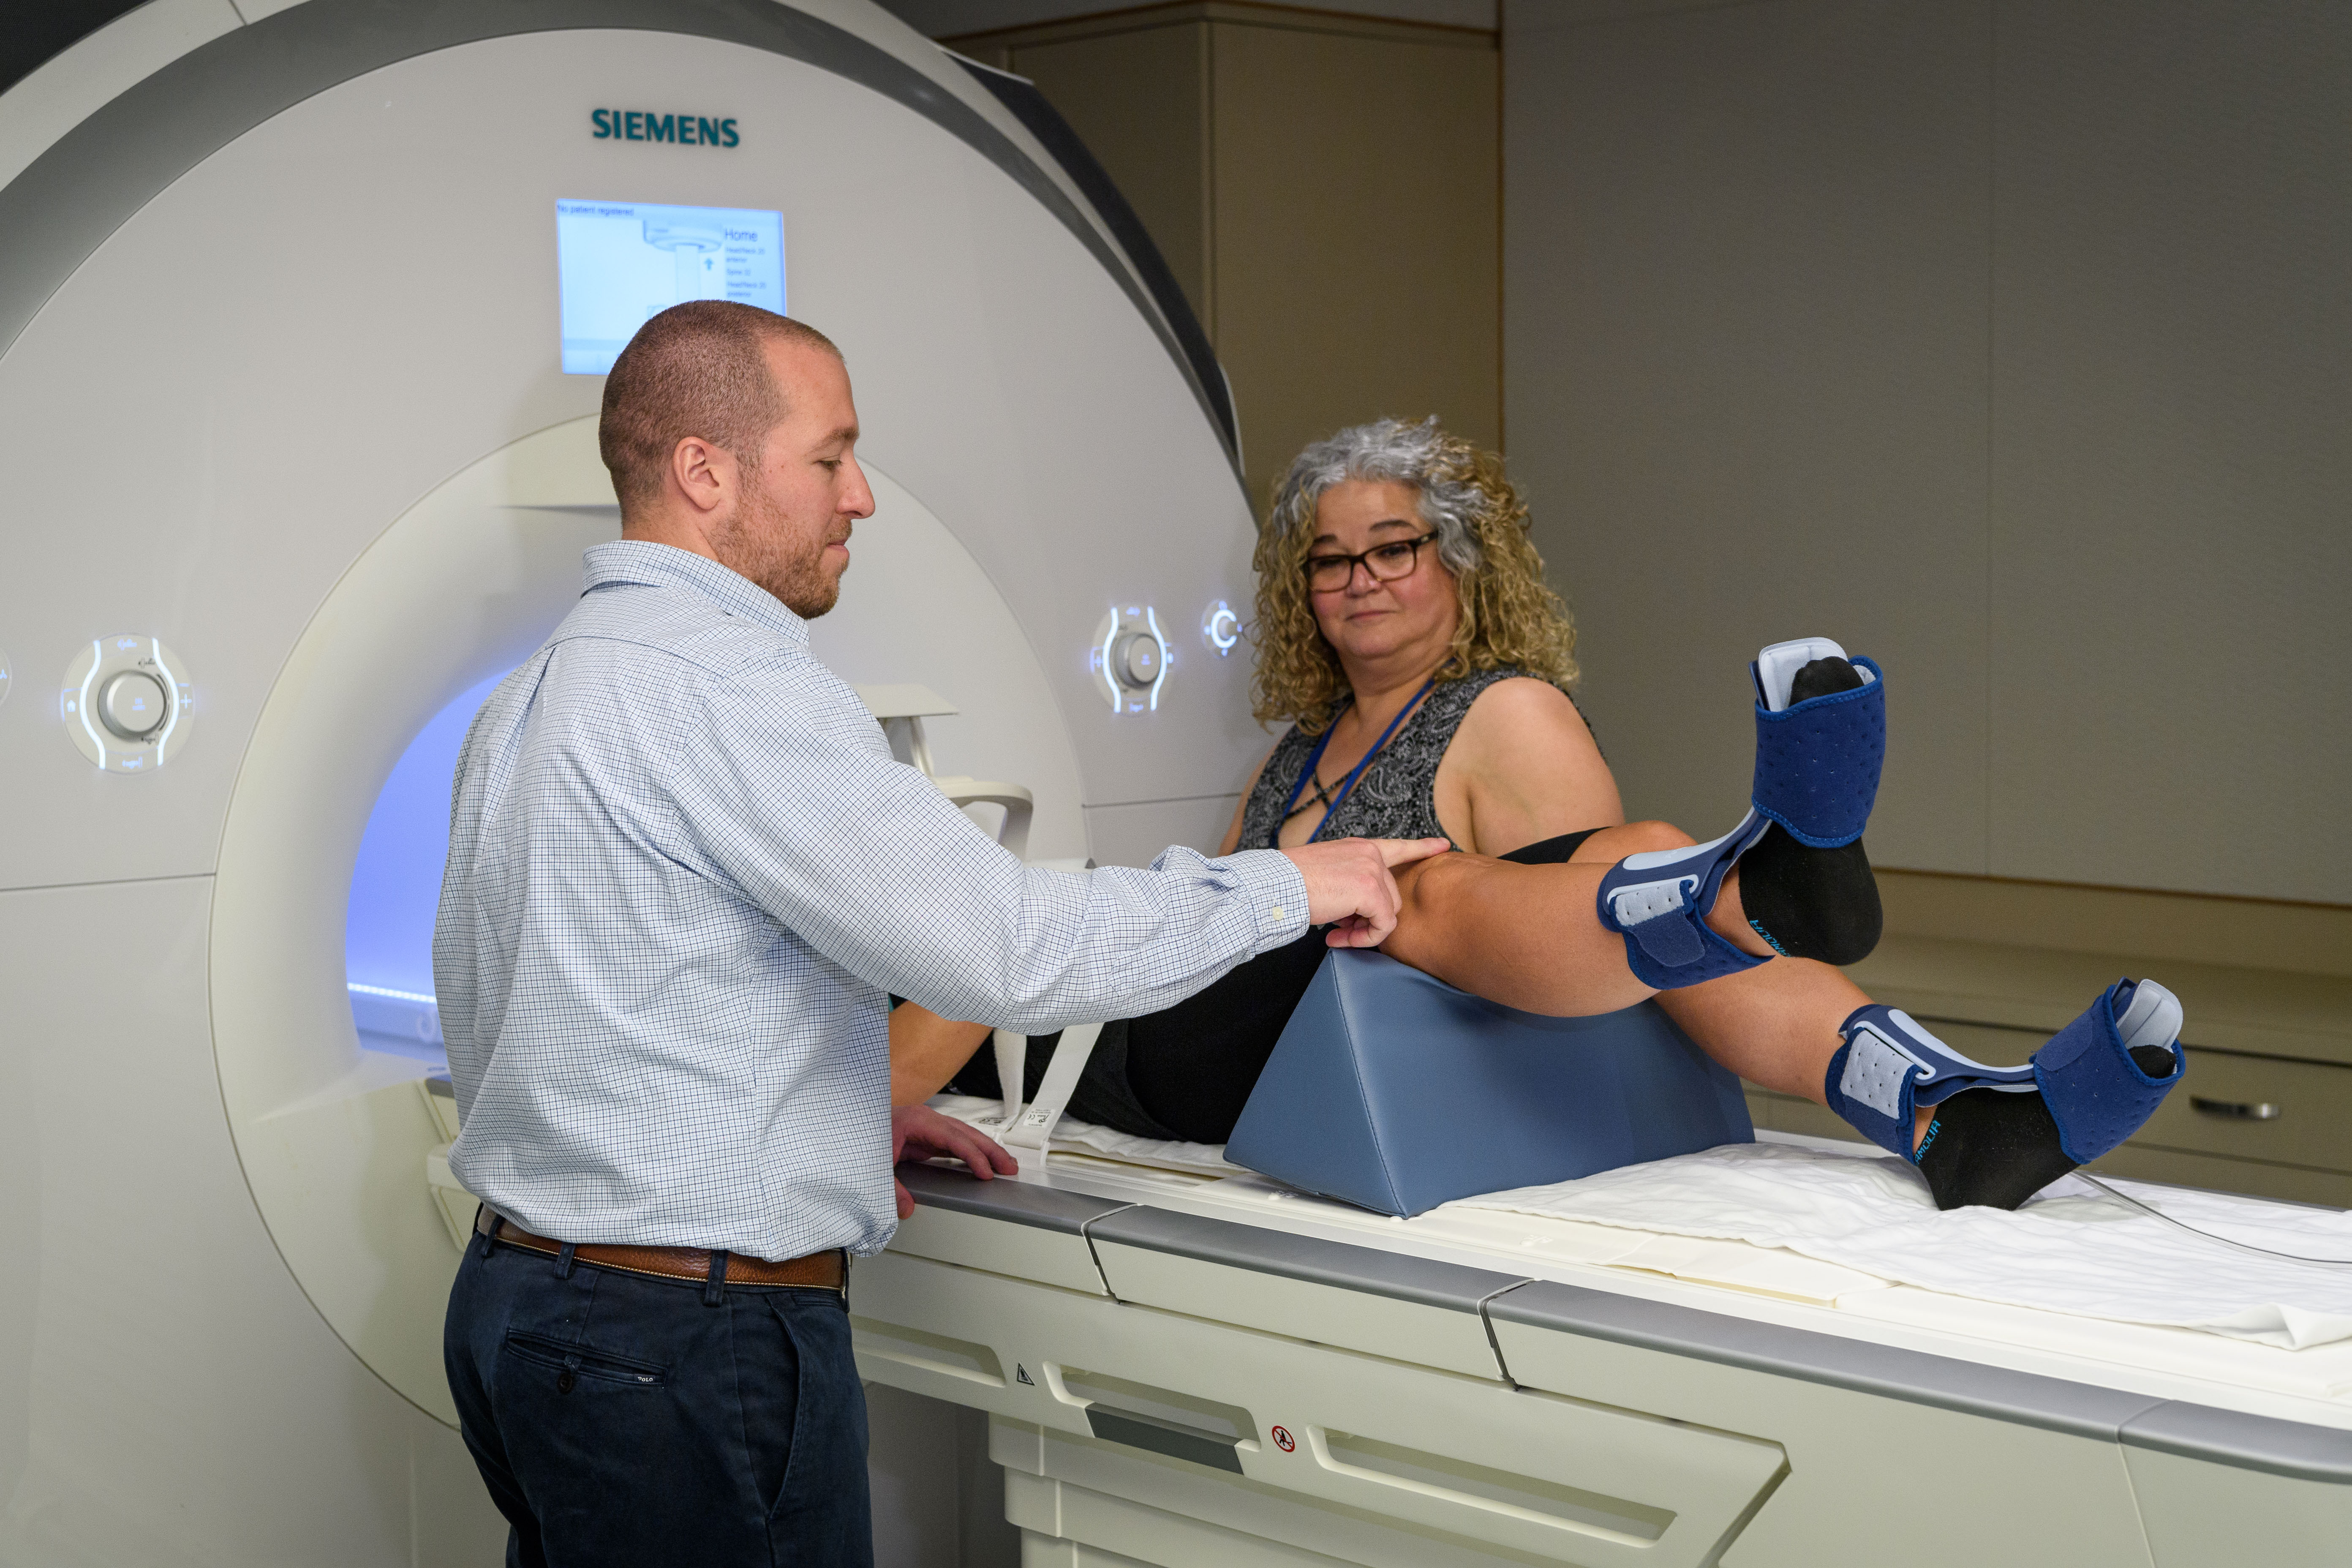
\includegraphics[height=.6\textheight]{img/acl1.jpg}
	\end{center}

\end{frame}

%%% Lepley 3

\begin{withoutheadline}\begin{frame}

	We also hope to examine the contribution of these neurophysiological outcomes to clinical measures of function defined as quadriceps muscle strength, knee joint biomechanics and self-reported disability.  
	
	\begin{center}
		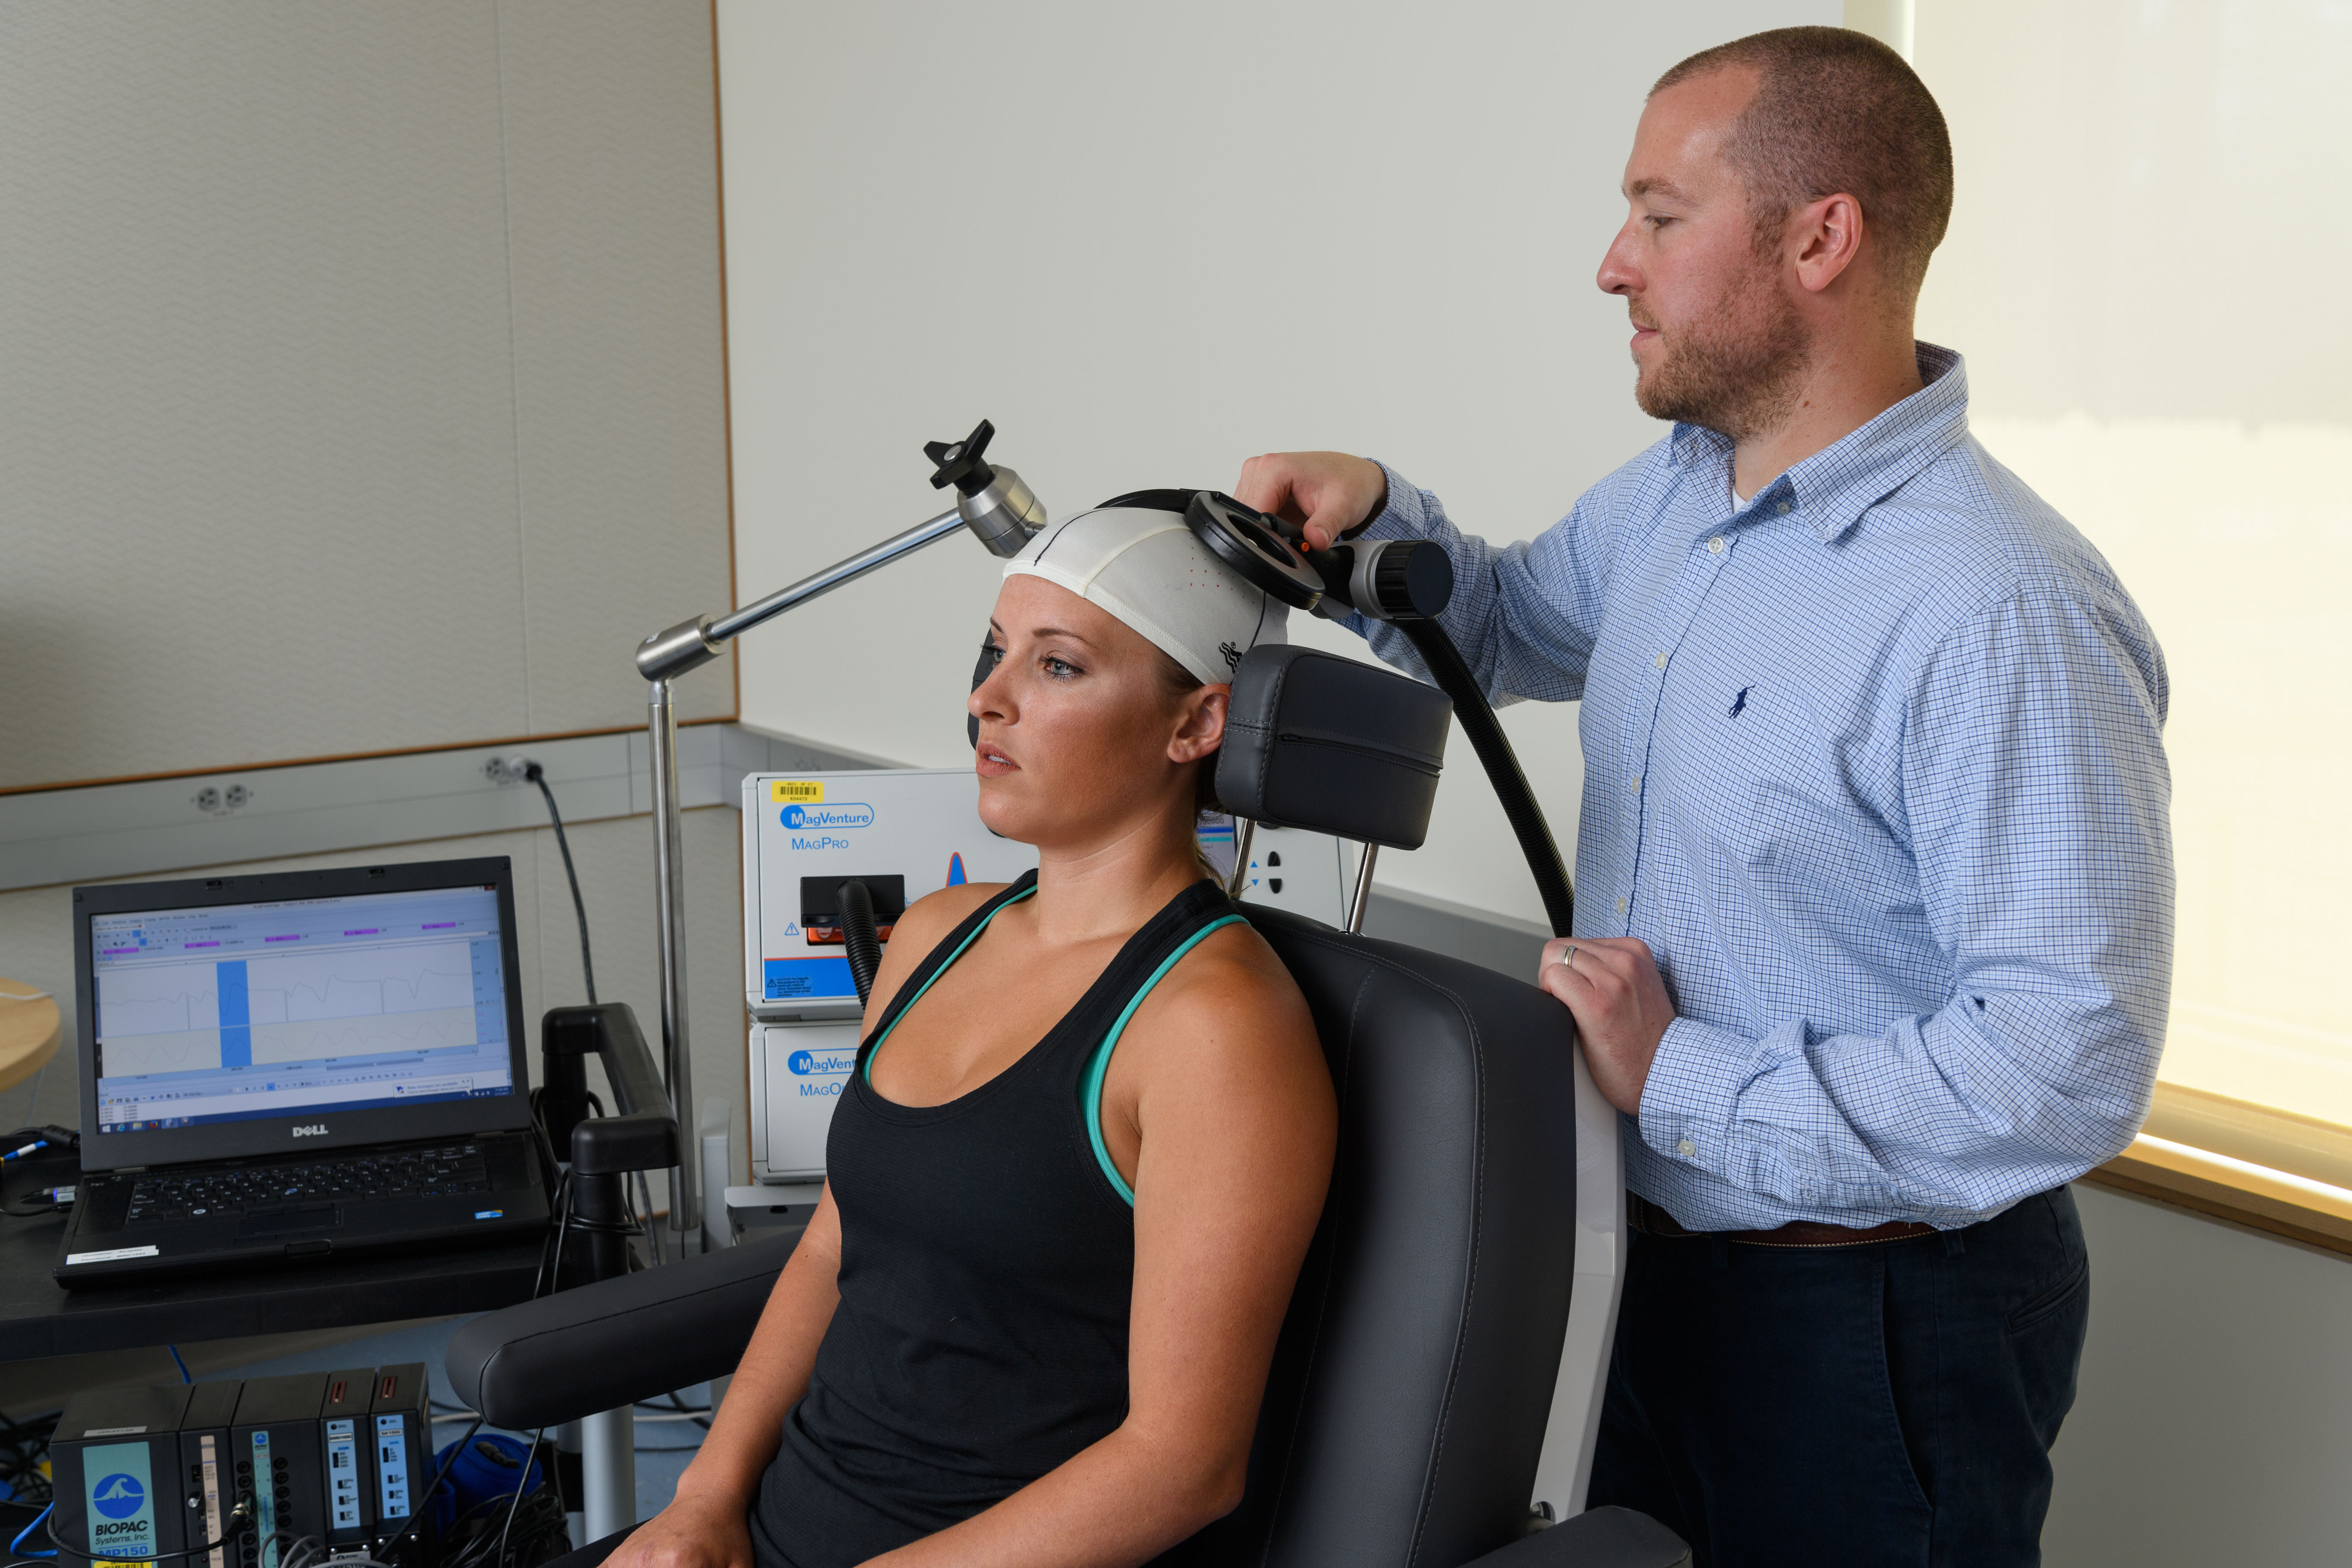
\includegraphics[height=.8\textheight]{img/acl2.jpg}
	\end{center}
\end{frame}\end{withoutheadline}

%%% Davis
\begin{frame}
	\frametitle{Charles Davis}
	\framesubtitle{IBRAiN Fellow}

	\begin{columns}[T]
		\begin{column}{.25\textwidth}
			% \begin{block}{}
			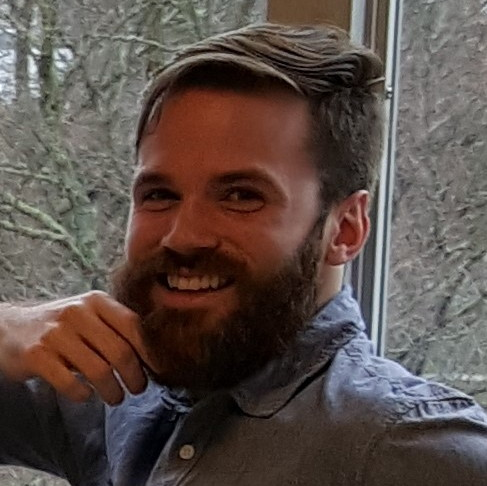
\includegraphics[width=\textwidth]{img/davis.jpg}
			%  \end{block}
		\end{column}

		\begin{column}{.75\textwidth}
			Grounded cognition theories suggest that our sensorimotor system is critical for high-level conceptual processing --- understanding coffee entails accessing its dark colour, its nutty smell, and so on. It remains unclear how such theories can accommodate abstract concepts like theory. We suspect that contextual information is critical for processing abstract concepts, and as such, we are examining whether the hippocampus is more involved when processing abstract concepts (as opposed to concrete ones) in context, and whether it works together with (i.e. shows functional connectivity with) high-level convergence zones like anterior temporal lobe. Such connectivity may facilitate the integration of contextual detail proposed to be necessary for processing abstract concepts like theory.
		\end{column}
	\end{columns}
\end{frame}

%%%% Ryherd
\begin{frame}
	\frametitle{Kayleigh Ryherd}
	\framesubtitle{IBRAiN Fellow}

	\begin{columns}[T]
		\begin{column}{.25\textwidth}
			% \begin{block}{}
			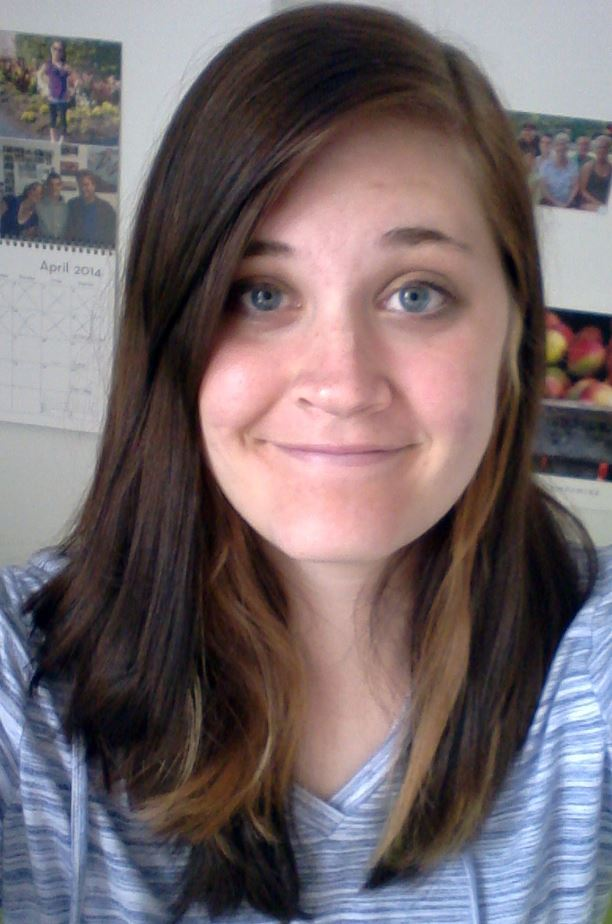
\includegraphics[width=\textwidth]{img/ryherd.jpg}
			%  \end{block}
		\end{column}

		\begin{column}{.75\textwidth}
			I am studying the neural underpinnings of category learning. Specifically, I will compare how we learn dense categories, which have many correlated features, to how we learn sparse categories, which are defined based on a single feature. I will also investigate how learning these different types of categories relates to reading comprehension ability.
		\end{column}
	\end{columns}
\end{frame}

%%%% Ryherd Poster
\begin{withoutheadline}\begin{frame}

	\begin{center}
		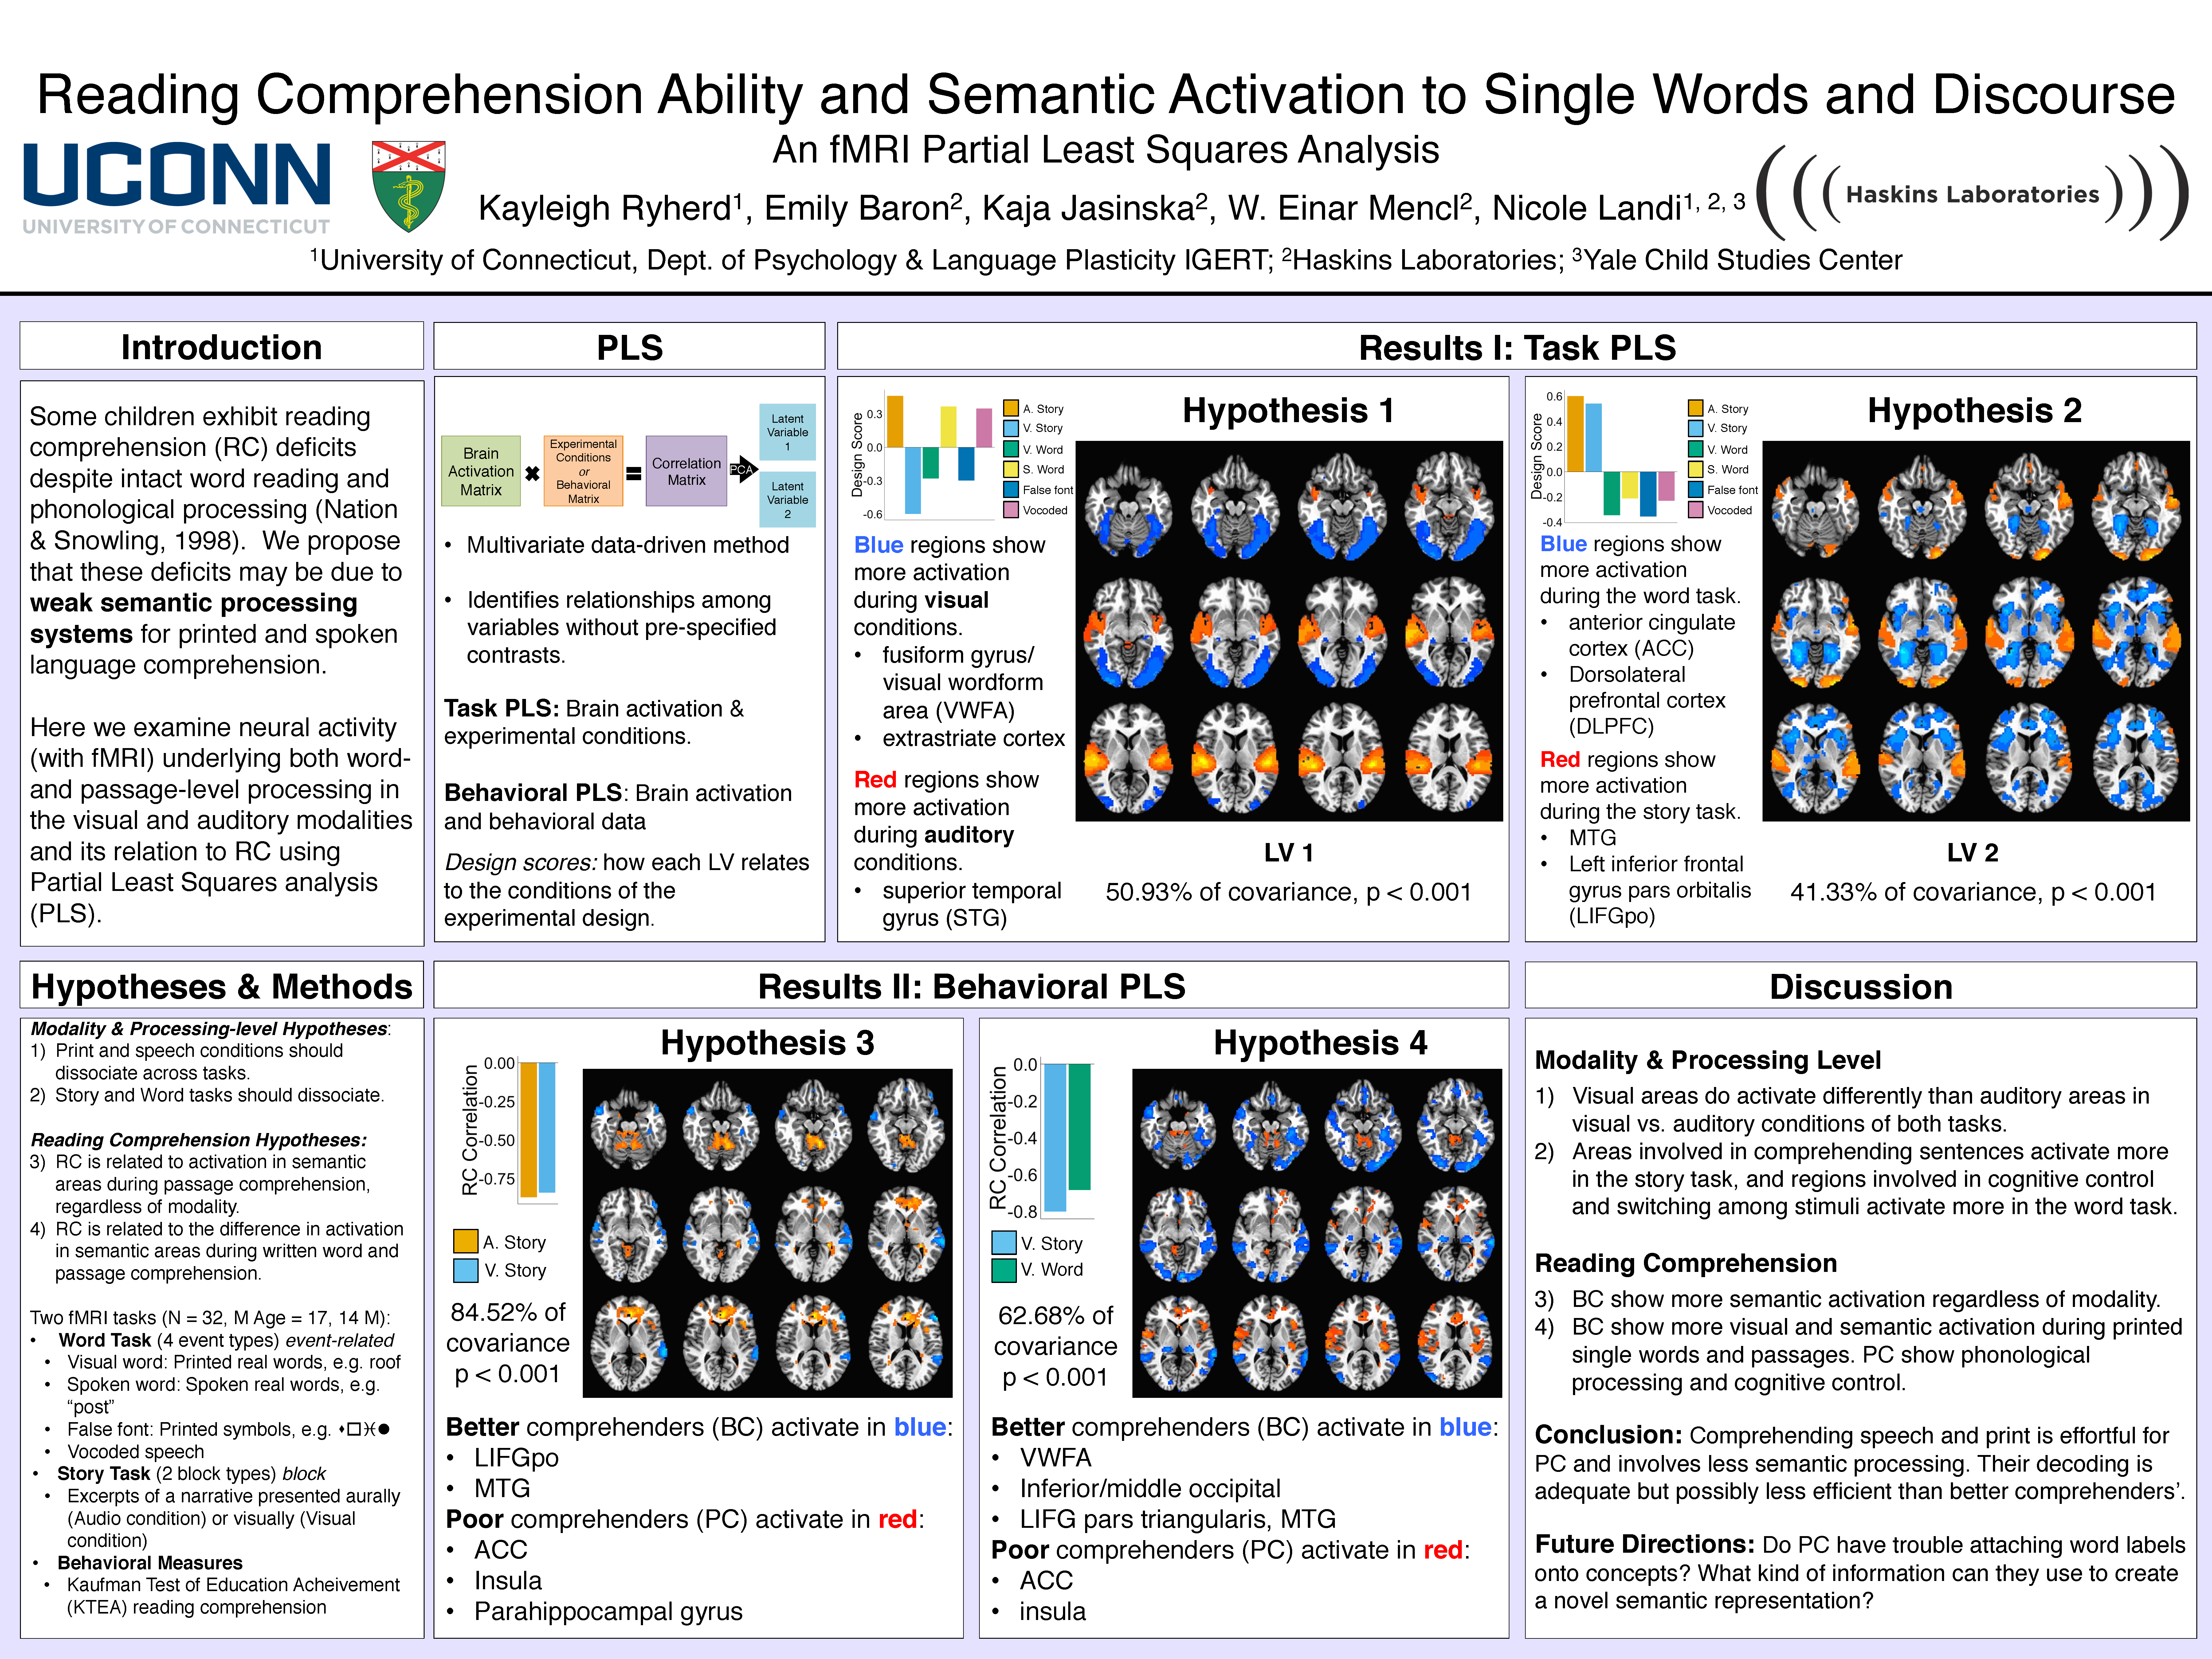
\includegraphics[height=.98\paperheight]{img/SNL_2015_Ryherd.pdf}
	\end{center}
\end{frame}\end{withoutheadline}

%%%% Ryherd Poster
\begin{withoutheadline}\begin{frame}

	\begin{center}
		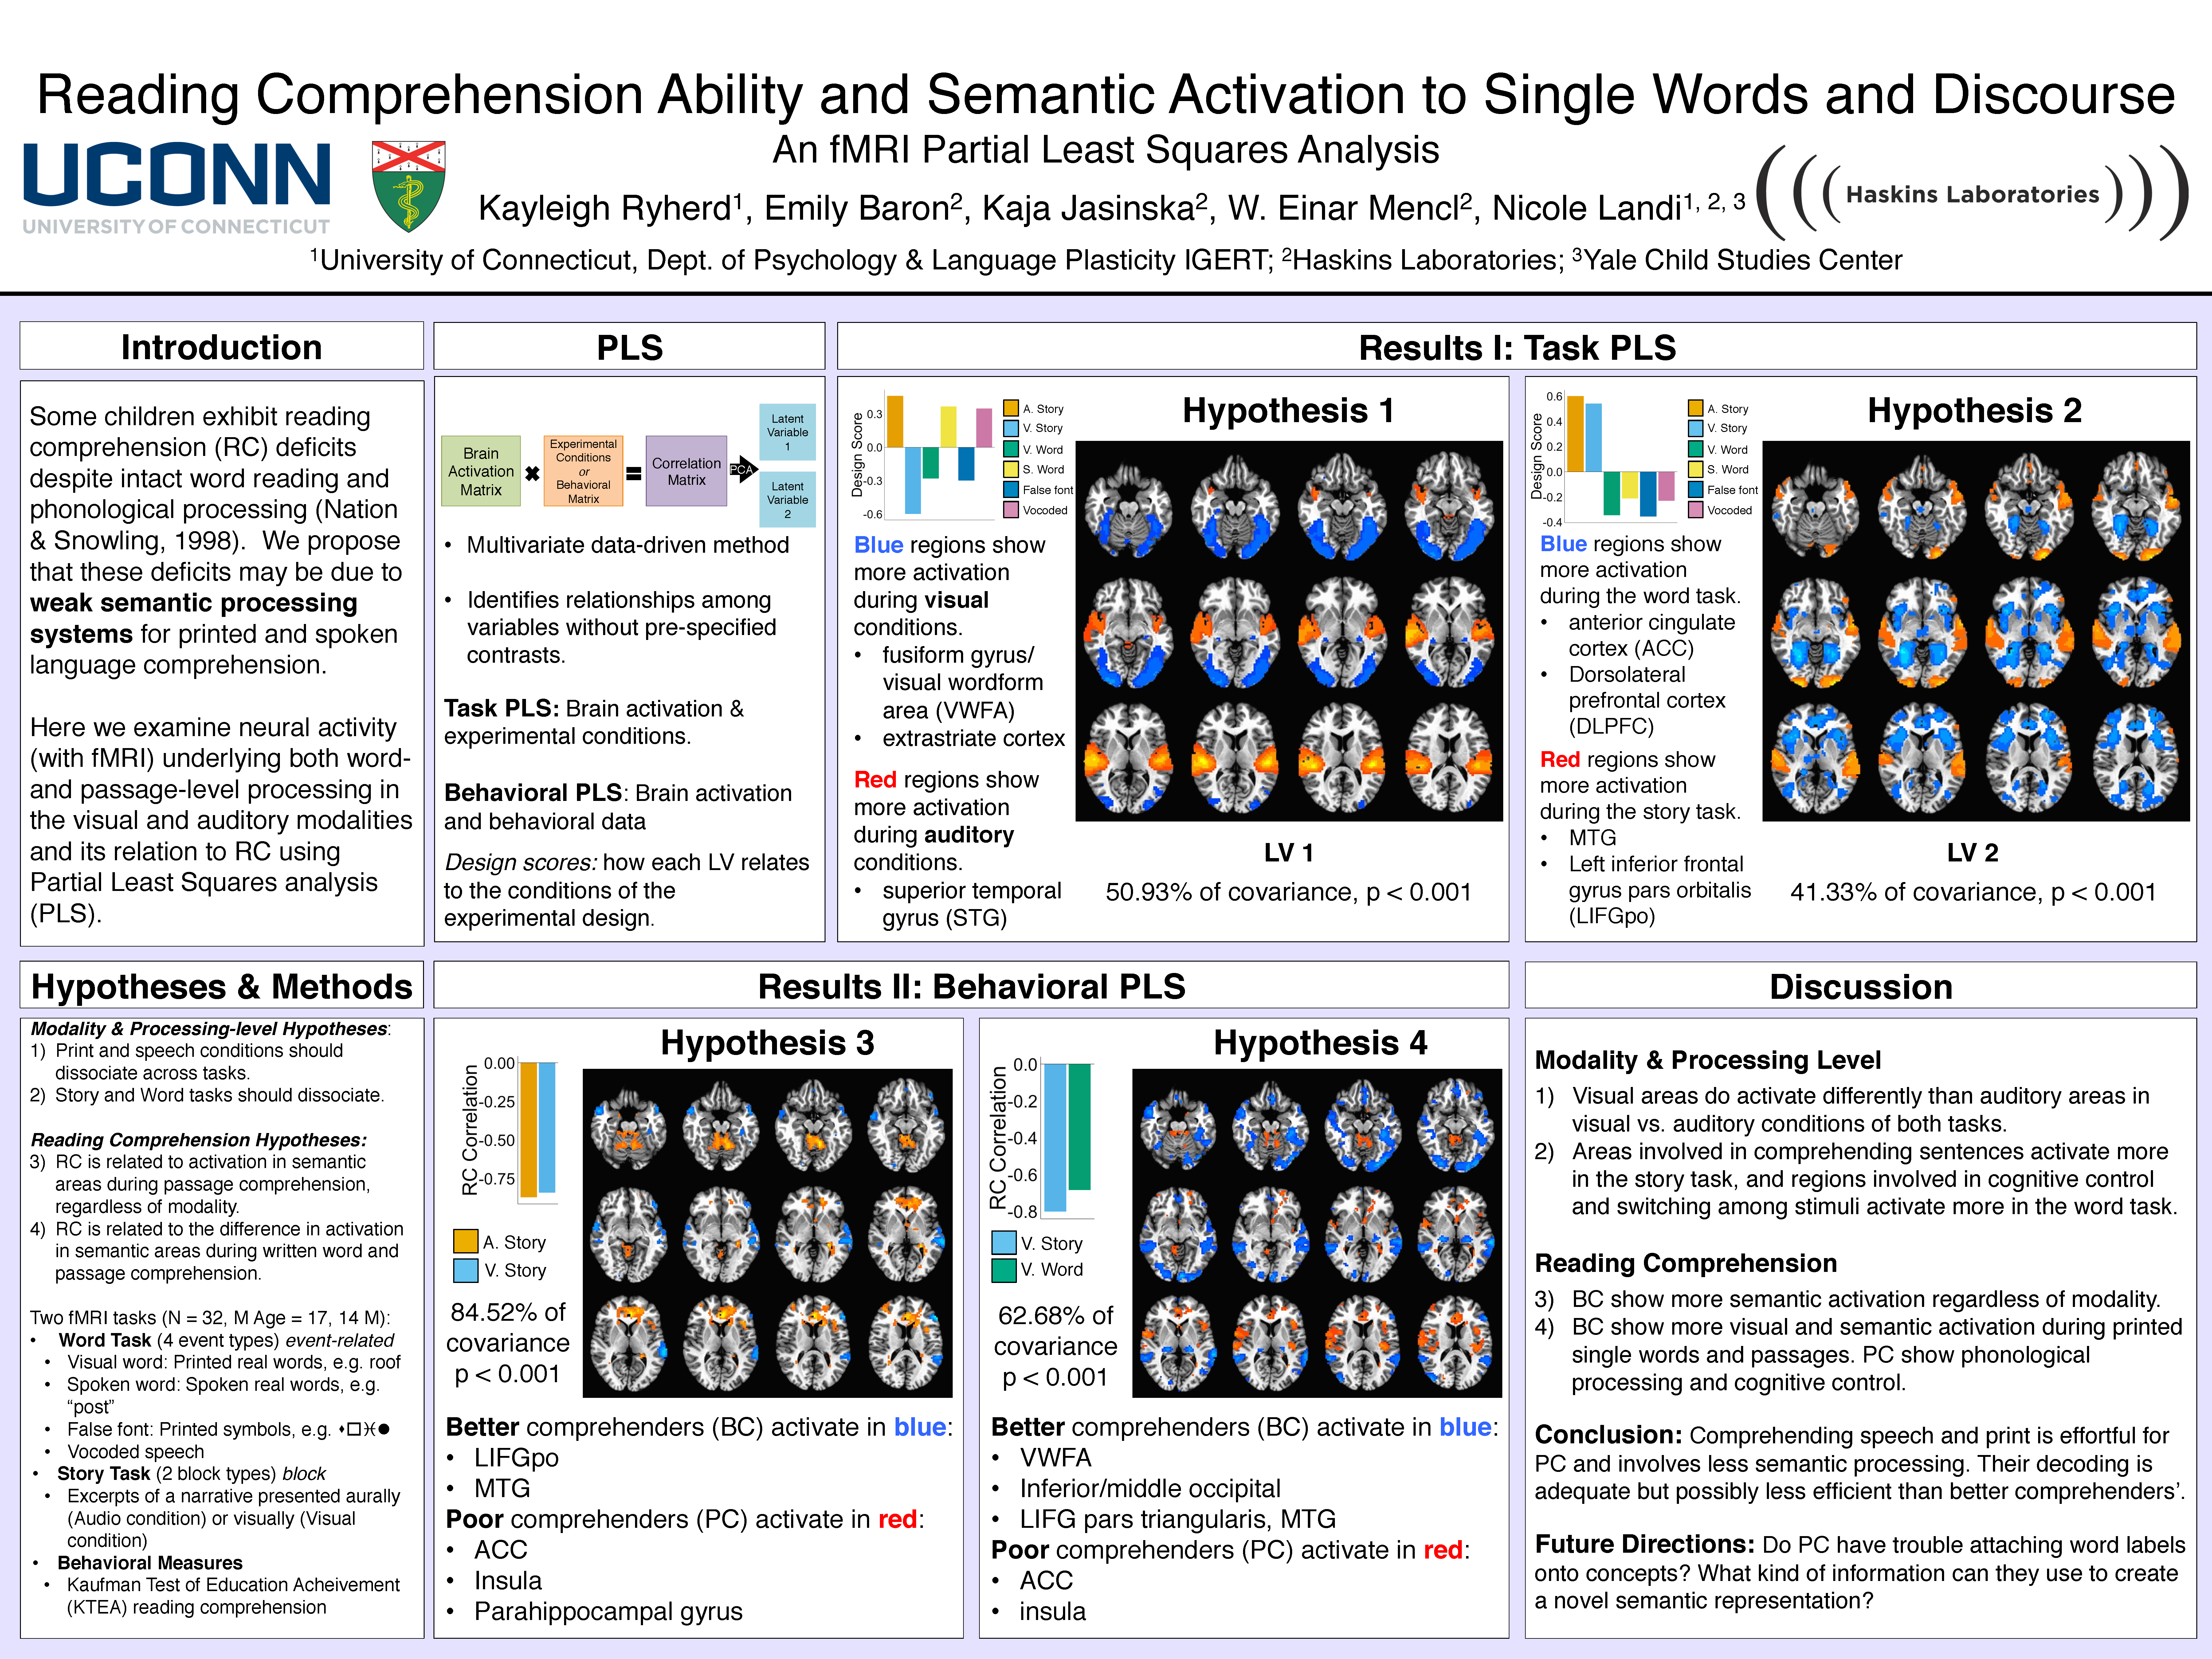
\includegraphics[height=.98\paperheight]{img/SNL_2015_Ryherd.pdf}
	\end{center}
\end{frame}\end{withoutheadline}


%%% Castelluccio
\begin{frame}
	\frametitle{Brian Castelluccio}
	\framesubtitle{NSF-IGERT Training Fellow}

	\begin{columns}[T]
		\begin{column}{.25\textwidth}
			% \begin{block}{}
			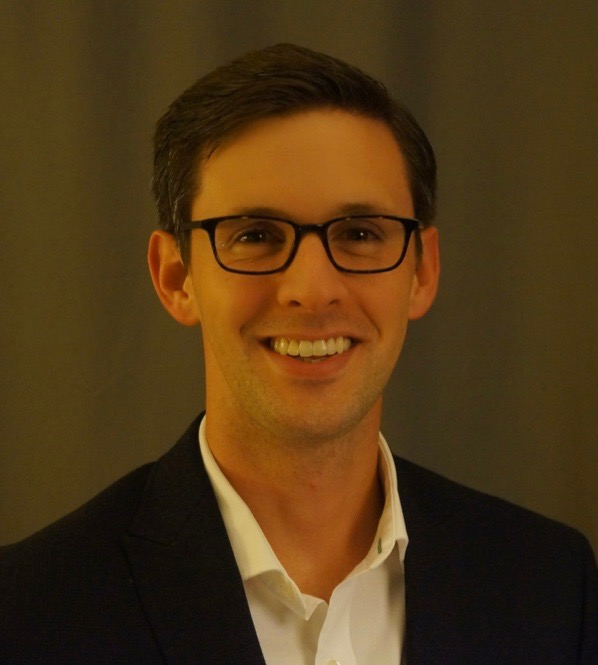
\includegraphics[width=\textwidth]{img/castelluccio.jpg}
			%  \end{block}
		\end{column}

		\begin{column}{.75\textwidth}
			Language acquisition is a complex generalization task that requires prolific extension of learned form-to-meaning mappings to novel stimuli. Generalization itself, the process by which abstracted features of past experiences are extended to new instances, is an area of relative weakness in autism spectrum disorder. I aim to determine whether linguistic generalization in particular is an area of weakness for people with autism spectrum disorder and to compare the neural resources engaged for linguistic generalization in people with and without autism.
		\end{column}
	\end{columns}
\end{frame}

%%% Ly
\begin{frame}
	\frametitle{Monica Ly}
	\framesubtitle{IBRAiN Fellow}

	\begin{columns}[T]
		\begin{column}{.25\textwidth}
			% \begin{block}{}
			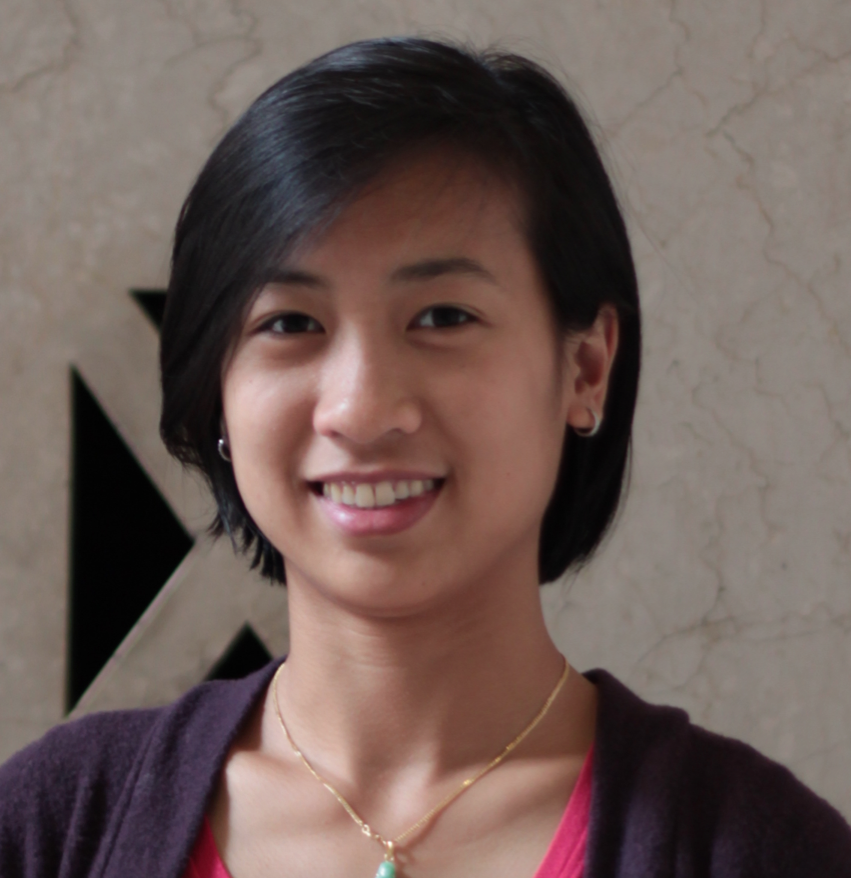
\includegraphics[width=\textwidth]{img/ly.png}
			%  \end{block}
		\end{column}

		\begin{column}{.75\textwidth}
			In collaboration with the BrainScope study, I aim to conjoin rs-MRI and DTI results to develop a machine learning algorithm to classify mild traumatic brain injury from no injury; this algorithm will distinguish recently concussed athletes from matched controls.
		\end{column}
	\end{columns}
\end{frame}

%%% Michaels
\begin{frame}
	\frametitle{Tim Michaels}
	\framesubtitle{IBRAiN Fellow}

	\begin{columns}[T]
		\begin{column}{.25\textwidth}
			% \begin{block}{}
			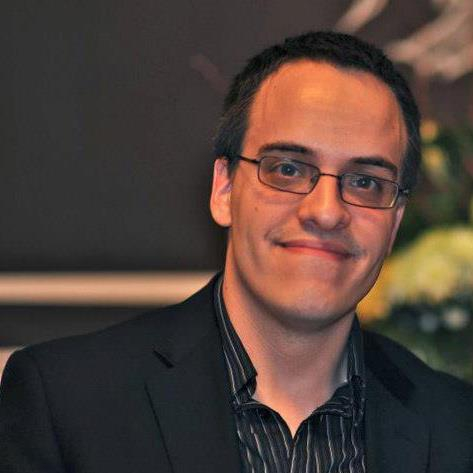
\includegraphics[width=\textwidth]{img/ProfileTM.jpg}
			%  \end{block}
		\end{column}

		\begin{column}{.75\textwidth}
			Millions of individuals with serious mental illness do not respond to currently available treatments. It is still unclear how differences in the brain contribute to symptoms of mental illness such as memory problems, concentration difficulties and hearing voices. I study how the brain works in those who experience such symptoms and those who do not. By providing a better understanding of how the brain operates in psychiatric disease, I hope to develop improved treatments for those suffering from mental illness. 

		\end{column}
	\end{columns}
\end{frame}

%%%% Myers
\begin{frame}
	\frametitle{Emily Myers}
	\framesubtitle{Associate Professor\\ \textit{Department of Speech, Language, and Hearing Sciences} }

	\begin{columns}[T]
		\begin{column}{.25\textwidth}
			% \begin{block}{}
			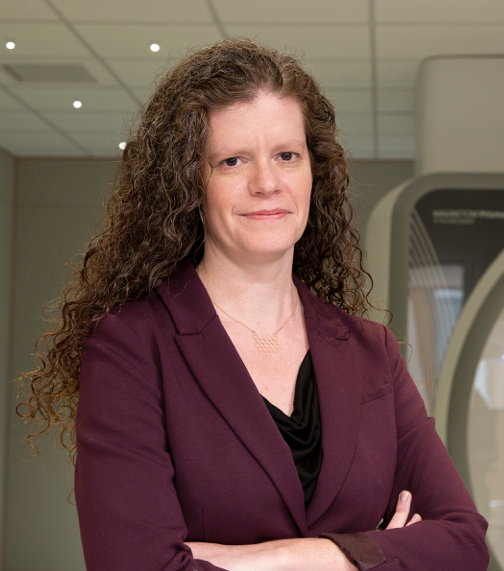
\includegraphics[width=\textwidth]{img/myers.png}
			%  \end{block}
		\end{column}

		\begin{column}{.75\textwidth}
			Studies of second language learning usually use tasks with explicit feedback to help listeners learn non-native speech sounds. However, implicit learning paradigms might more closely resemble real language learning situations. In this study, we use an implicit learning paradigm to teach participants to discriminate two very similar non-native speech sounds. We use fMRI to ask whether these new sounds recruit the same brain areas as native language speech processing.
		\end{column}
	\end{columns}
\end{frame}

%%% Luthra
\begin{frame}
	\frametitle{Sahil Luthra and Pam Fuhrmeister}
	\framesubtitle{NSF IGERT Fellows}

	\begin{columns}[T]
		\begin{column}{.25\textwidth}
			% \begin{block}{}
			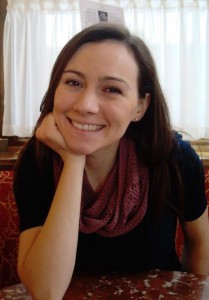
\includegraphics[height=.5\textheight]{img/Fuhrmeister.jpg}

			
\includegraphics[height=.5\textheight]{img/Luthra.jpg}
			%  \end{block}
		\end{column}

		\begin{column}{.75\textwidth}
			The Myers Lab is investigating how different brain regions (and frontal regions in particular) support the acquisition of non-native speech sounds. We scanned native English speakers before and after three days of training on a Hindi sound contrast that is difficult for English speakers to perceive. We are currently analyzing our functional and DTI data to examine how functional and structural differences between participants predict how well they learned these sounds.
		\end{column}
	\end{columns}
\end{frame}

%%% Hancock
\begin{frame}
	\frametitle{Roeland Hancock}
	\framesubtitle{Associate Director, \textit{BIRC} \\
	Assistant Research Professor, \textit{Department of Psychological Sciences} }

	\begin{columns}[T]
		\begin{column}{.25\textwidth}
			% \begin{block}{}
			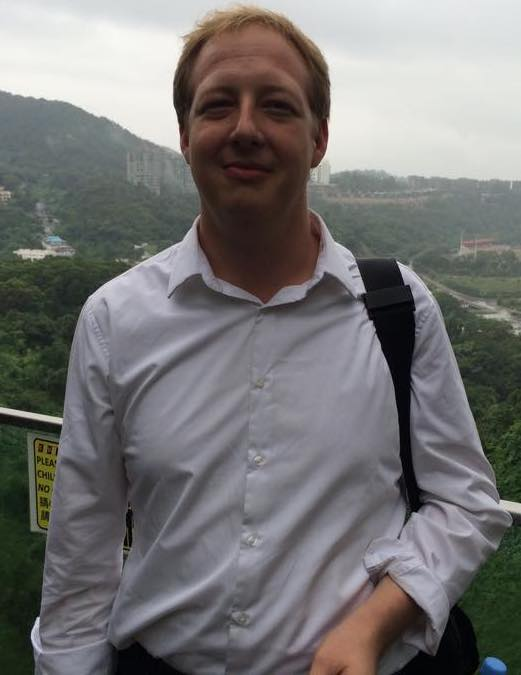
\includegraphics[width=\textwidth]{img/hancock.jpg}
			%  \end{block}
		\end{column}

		\begin{column}{.75\textwidth}
			Dr. Hancock is interested in the neurobiological factors underlying individual variability in language processing and the application of new mathematical and computational techniques to understanding these processes. His current research interests include the use of magnetic resonance spectroscopy to study neural excitability in auditory and language processing; distinguishing genetic and environmental contributions to language pathways; and developing tablet-based games for cognitive and literacy assessment. 
		\end{column}
	\end{columns}
\end{frame}
\end{document}